\documentclass[conference]{IEEEtran}

\usepackage[ruled,vlined,linesnumbered]{algorithm2e}
\usepackage{booktabs}
\usepackage[hang]{caption}
\usepackage{cite}
\usepackage{flushend}
\usepackage[bottom,hang]{footmisc}
\usepackage[T1]{fontenc}
\usepackage[utf8]{inputenc}
\usepackage{graphicx}
\usepackage{icomma}
\usepackage{listings}
\usepackage{newtxtext}
\usepackage{newtxmath}
\usepackage{textgreek}
\usepackage{url}
\usepackage{xcolor}
\RequirePackage[l2tabu, orthodox]{nag}

% Allow PDF 1.7 documents to be included with \includegraphics
\pdfminorversion=7

% Suppress "multiple pdfs with page group included in a single page" warning
\pdfsuppresswarningpagegroup=1

% Define colors for code highlighting
\definecolor{color-bg}{HTML}{F6F8FA}
\definecolor{color-keyword}{HTML}{D73A49}
\definecolor{color-ident}{HTML}{005CC5}
\definecolor{color-string}{HTML}{032F62}
\definecolor{color-comment}{HTML}{6A737D}

% Listing
\lstset{%
  language={C++},
  basicstyle={\small\ttfamily},%
  backgroundcolor=\color{color-bg},%
  identifierstyle={\small\ttfamily},%
  commentstyle={\small\itshape\color{color-comment}},%
  keywordstyle={\small\bfseries\color{color-ident}},%
  % ndkeywordstyle={\small\ttfamily},%
  stringstyle={\small\ttfamily\color{color-string}},%
  frame={trbl},%
  frameround={tttt},%
  breaklines=true,%
  columns=[l]{fullflexible},%
  numbers=left,%
  numberstyle={\scriptsize},%
  stepnumber=1,%
  numbersep=1em,%
  % lineskip=-0.5ex,%
  mathescape,%
  xleftmargin=2em,%
  framexleftmargin=1.5em,%
}

\begin{document}

% algorithme2
\SetKwFor{PFor}{parallel for}{do}{end}

\title{kEDM: A Performance-portable Implementation of Empirical Dynamical Modeling}

\author{%
    \IEEEauthorblockN{%
        Keichi Takahashi,\\Wassapon Watanakeesuntorn,\\Kohei Ichikawa
    } \\
    \IEEEauthorblockA{%
        Nara Institute of Science and Technology\\
        Nara, Japan\\
        \{keichi, wassapon.watanakeesuntorn.wq0,\\ ichikawa\}@is.naist.jp
    }
    \and
    \IEEEauthorblockN{%
        George Sugihara
    } \\
    \IEEEauthorblockA{%
        University of California San Diego\\
        California, USA\\
        gsugihara@ucsd.edu
    }
    \and
    \IEEEauthorblockN{%
        Gerald M. Pao
    } \\
    \IEEEauthorblockA{%
        Salk Institute for Biological Studies\\
        California, USA\\
        pao@salk.edu
    }
}

\maketitle

\begin{abstract}
    Recent rapid scale out of high performance computing systems has
    rapidly and continuously increased the scale and complexity of the
    interconnects. As a result, current static and over-provisioned
    interconnects are becoming cost-ineffective. Against this background, we have
    been working on the integration of network programmability into
    the interconnect control, based on the idea that dynamically controlling
    the packet flow in the interconnect according to the communication pattern
    of applications can increase the utilization of interconnects and improve
    application performance. Interconnect simulators come in handy especially
    when investigating the performance characteristics of interconnects with
    different topologies and parameters. However, little effort has been put
    towards the simulation of packet flow in dynamically controlled interconnects,
    while simulators for static interconnects have been extensively researched
    and developed. To facilitate analysis on the performance
    characteristics of dynamic interconnects, we have developed PFAnalyzer.
    PFAnalyzer is a toolset composed of PFSim, an interconnect simulator
    specialized for dynamic interconnects, and PFProf, a profiler.
    PFSim allows interconnect researchers and designers to investigate
    congestion in the interconnect for an arbitrary cluster configuration and
    a set of communication patterns collected by PFProf. PFAnalyzer is used
    to demonstrate how dynamically controlling the interconnects can reduce
    congestion and potentially improve the performance of applications.
\end{abstract}

\begin{IEEEkeywords} Simulation, Profiling, Interconnect, Message Passing Interface, Software
    Defined Networking
\end{IEEEkeywords}

\section{Introduction}

Empirical Dynamical Modeling (EDM)~\cite{Chang2017} is a...

\cite{Ma2017}

brain science~\cite{Natsukawa2017}

We have been developing mpEDM~\cite{mpedm}, a massively parallel
implementation of EDM.

Create a performance-portable implementation of EDM for both CPU and GPU
platforms.

\clearpage

\section{Background}

\begin{figure*}
    \centering
    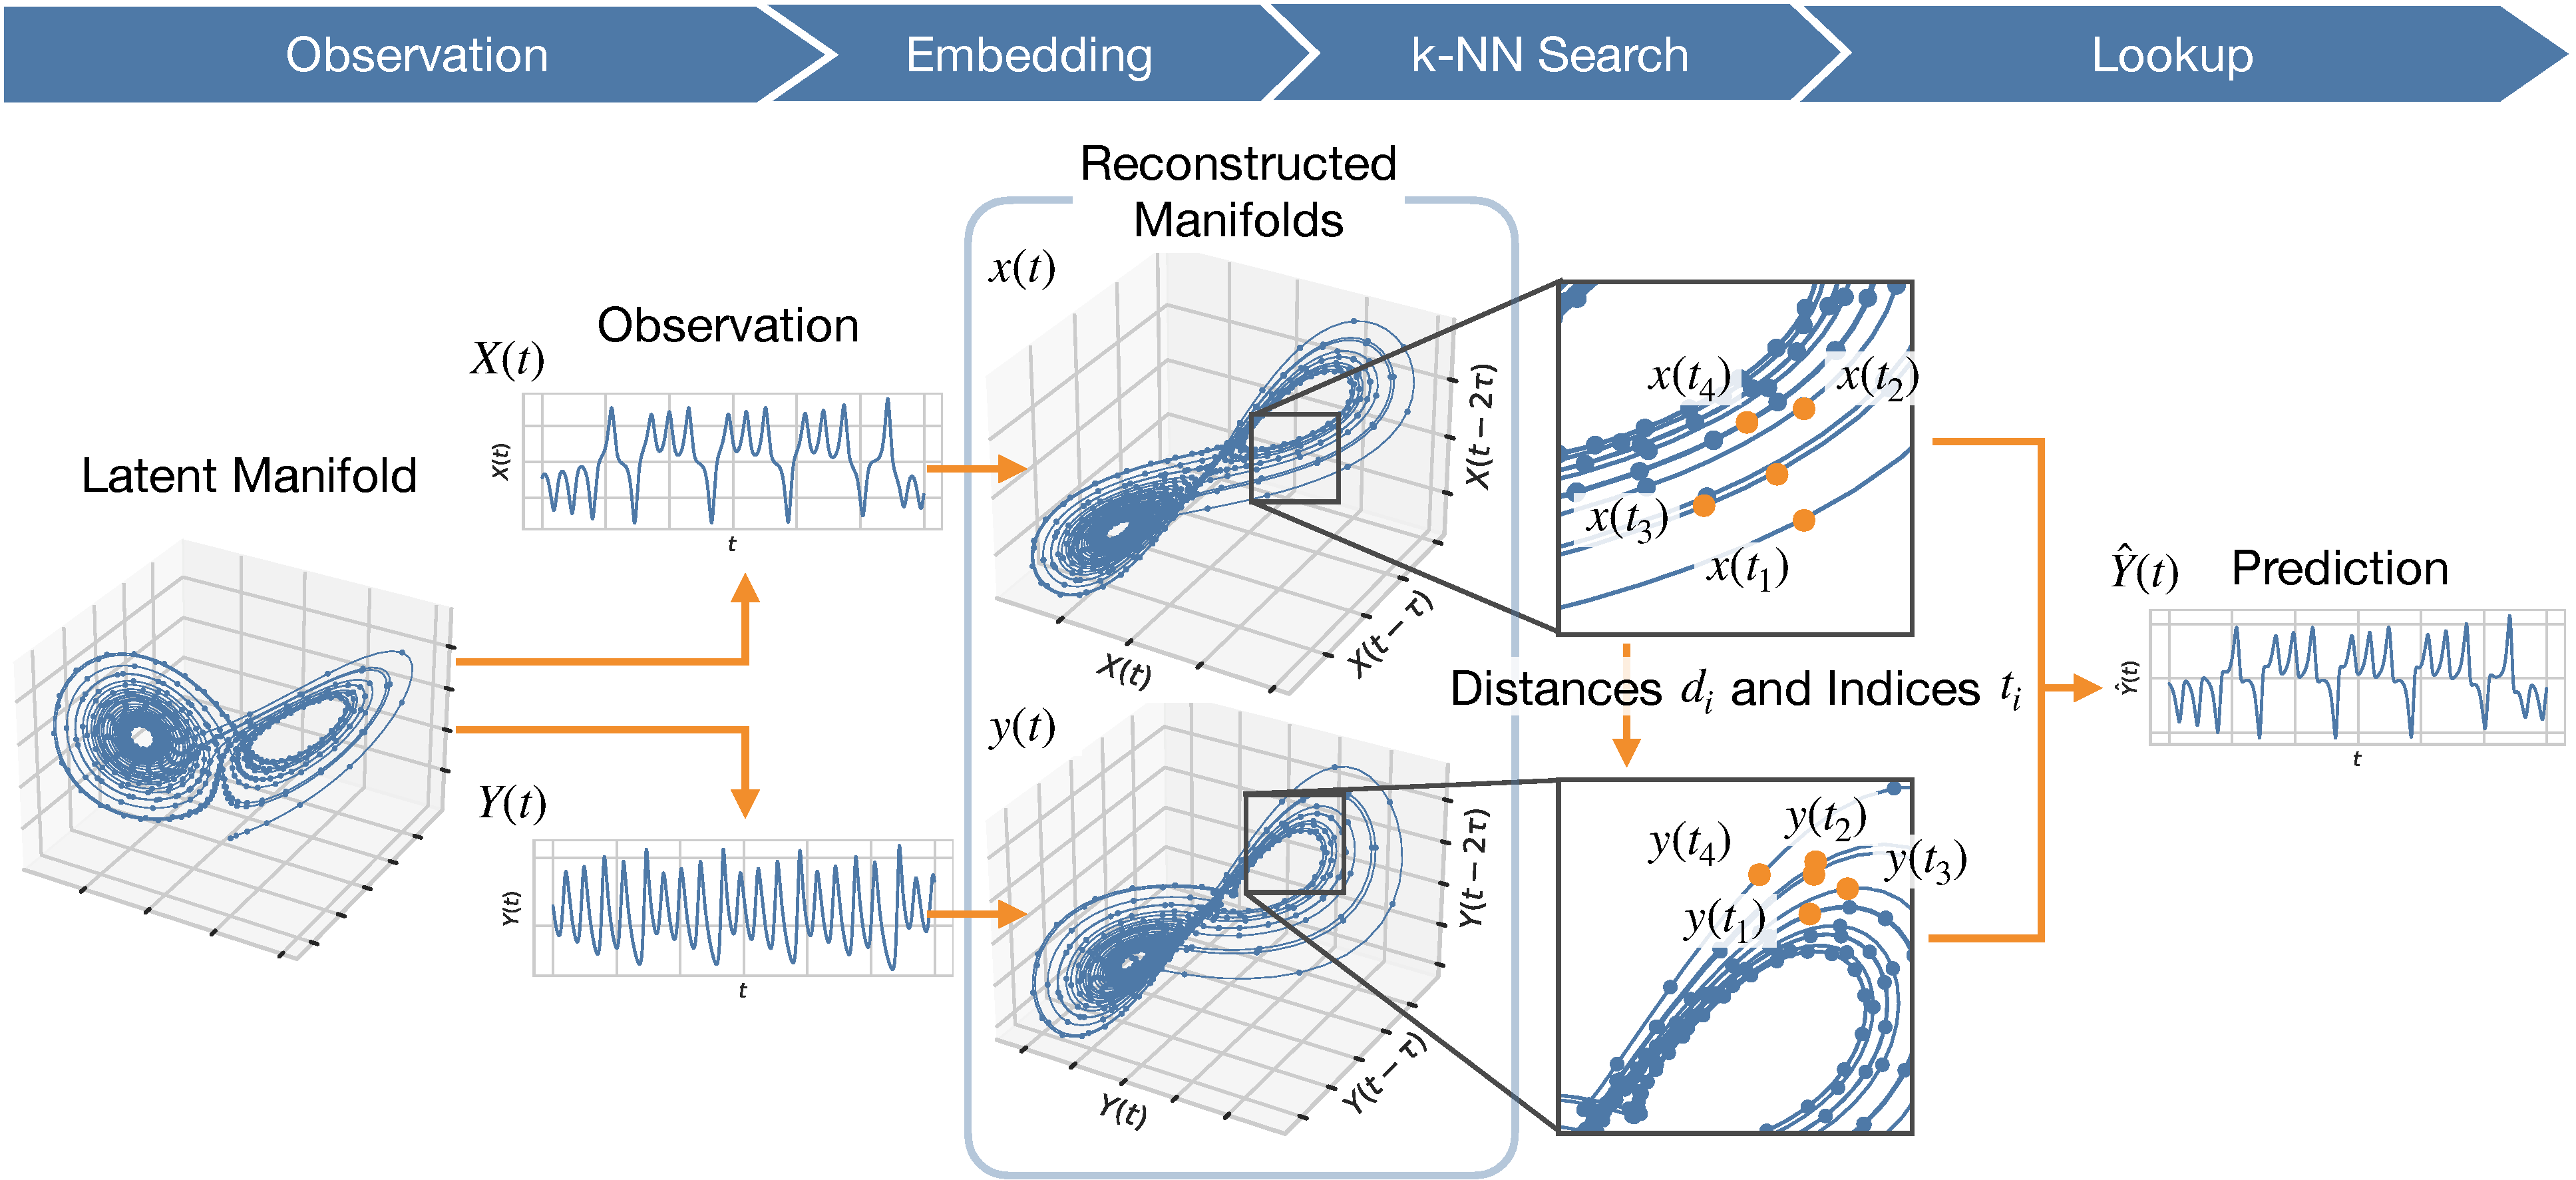
\includegraphics{figs/xmap_overview}
    \caption{Overview of EDM cross mapping}%
    \label{fig:edm}
\end{figure*}

\subsection{Empirical Dynamical Modeling (EDM)}

\subsection{Challenges in mpEDM}\label{sec:challenges}

This subsection discusses the two major challenges in mpEDM: performance
portability and flexibility.

\subsubsection{Performance portability}

mpEDM was based on ArrayFire~\cite{Malcolm2012}, a general purpose library for
GPU computing. We chose ArrayFire primarily for its productivity and
portability. ArrayFire provides CUDA and OpenCL backends to run on OpenCL
devices. It also provides a CPU backend. Unfortunately, most of the functions
provided by the CPU backend are neither multi-threaded or vectorized. For this
reason, we implemented our implementation for CPU\@.

As a result, mpEDM had a ArrayFire-based GPU implementation and a CPU-based
implementation of EDM, doubling the maintenance cost. Considering the
diversifying target hardware, we wish a unified implementation that achieves
consistent and reasonable performance across a diverse set of hardware.

\subsubsection{Flexibility}

Since mpEDM was relying on ArrayFire's k-nearest neighbor search function
(\texttt{nearestNeighbour()}), we were unable to modify nor tune the k-NN
search to suit our use case and missed opportunities for further optimization.
ArrayFire's nearest neighbor function accepts two input arrays, which are the
reference and query points, and returns a list of closest reference points and
their distances for each query point. This interface is simple and
easy-to-use. However, when applying to EDM, the time-delayed embedding needs
to be performed on CPU in advance and passed to ArrayFire. This hinders
performance because it increases the amount of data that needs to be read from
GPU memory.

Another potential optimization opportunity is the partial sort function
\texttt{topk()} invoked in the k-NN search. ArrayFire uses NVIDIA's
CUB\footnote{\url{https://nvlabs.github.io/cub/}} library to implement partial
sort. CUB is a highly optimized library and being used by other libraries such
as Thrust\footnote{\url{https://github.com/NVIDIA/thrust}}. ArrayFire's
\texttt{topk()} function divides the input array into equal sized sub-array
and then calls CUB's \texttt{BlockRadixSort()} function to sort each
sub-array. It then extracts the top-$k$ elements from each sub-array and
concatenates them into a new array. This is recursively repeated until the
global top-$k$ elements are found. Even though this implementation is
well-optimized, it may not be optimal for EDM since the targeted $k$ is
relatively small ($\leq 20$).

Finally, we were unable to implement lookups efficiently on GPU using
ArrayFire. ArrayFire provides a construct called \textit{GFOR} that allows one
to perform embarrassingly parallel for-loops in parallel. Although we were
able to implement lookups using GFOR, the attained performance was poor. It
was also challenging to reduce memory consumption and memory copies because
ArrayFire implicitly allocates, deallocates and copies arrays.

\section{kEDM}

\subsection{Overall Design}

kEDM\footnote{\url{https://github.com/keichi/kEDM}} is a performance-portable
implementation of EDM based on Kokkos.

\subsection{Kokkos}

Kokkos~\cite{Edwards2014} is a performance portability framework developed at
the Sandia National Laboratories. It provides an abstraction layer that hides
the differences between low-level programming models such as OpenMP, CUDA,
ROCm and exposes a high-level C++ interface to the programmer. Using Kokkos,
it is possible to develop a cross-platform and performance-portable
application on a single source code base.

In Kokkos, the programmer specifies (1) the parallel pattern, (2) execution
policy, and (3) computational body of a loop. The parallel pattern includes
parallel-for, parallel-reduce and parallel-scan in the current release of
Kokkos. The execution policy defines how a loop is executed.
\texttt{RangePolicy}
Finally, the computational body is given as a C++ 11 lambda function.

Hierarchical parallelism: Allows one to exploit the hierarchy in a
    platform. Additionally, provides an interface to use high-speed
    team/thread scratch memory.

Listing~\ref{lst:basic} shows a AXPY kernel implemented in Kokkos.
In this example, the pattern is parallel-for.

\begin{lstlisting}[caption={Basic data parallel loop},label={lst:basic}]
Kokkos::parallel_for(RangePolicy<ExecSpace>(N),
KOKKOS_LAMBDA(int i) {
    y(i) = a * x(i) + y(i);
});
\end{lstlisting}

Listing~\ref{lst:hierarchical} shows a GEMV kernel using hierarchical
parallelism.

\begin{lstlisting}[caption={Hierarchical data parallel loop},label={lst:hierarchical}]
parallel_for(TeamPolicy<ExecSpace>(M),
KOKKOS_LAMBDA(const member_type &member) {
    int i = member.team_rank();
    float sum = 0.0f;

    parallel_reduce(TeamThreadRange(member, N),
    [=] (int j, float &tmp) {
        tmp += A(i, j) * x(j)
    }, sum);

    single(PerTeam(member),
    [=] () {
        y(i) = sum;
    });
});
\end{lstlisting}

\textit{View} is the fundamental data type in Kokkos and represents a
multidimensional array. Views are allocated explicitly by the user and
deallocated automatically by Kokkos using reference counting. A notable
feature of Kokkos view is that the layout of the multidimensional array is
parameterized. This frees programmers from tedious and error-prone index
calculation. Each view is associated to a memory space, an abstraction of
where the data resides. This includes Host, CUDA, CudaUVM, etc.

Execution space is an abstraction of where the code runs. The latest stable
release of Kokkos at the time of writing this paper supports Serial, OpenMP,
OpenMP Target, CUDA, ROCm, Pthread, HIP and HPX\@. A SYCL backend is in
development.

Both execution space and memory space are given as template parameters and
fixed at compile time, thereby making sure that accessing incompatible memory
at runtime does not happen.

Prior to implementing kEDM, we have examined a number of popular performance
portability frameworks. These include OpenMP, OpenACC, OpenCL and SYCL\@. We
chose Kokkos  because recent studies~\cite{Martineau2017, Deakin2019, Deakin2020}
have shown that it delivers portable performance on a large set of devices
compared to its alternatives. SYCL and OpenMP are attractive choices as they
have grown rapidly over the last few years in terms of hardware coverage and
delivered performance. However, we still consider them immature compared to
Kokkos at the point of writing this paper.

\subsection{All k-Nearest Neighbors Kernel}

We compose the All kNN search from two kernels: pairwise distance calculation
and partial sort.

As discussed in Section~\ref{sec:challenges}, performing the time-delayed
embedding into state space and then calculating the pairwise distances is
inefficient since it increases memory access. Instead, we perform the time
delayed embedding and distance calculation at the same time.

Algorithm~\ref{alg:distances} shows the pairwise distance calculation algorithm
in kEDM\@. A The outer most $i$-loop is parallelized using team parallel loop and
the $j$-loop is parallelized using intra-thread parallel loop. In addition, we
use the team-local scratch memory to cache $\mathrm{library}(k $\texttau$ + i)$
as it its referenced $LE$ times in each $i$-loop iteration.

\begin{algorithm}
    \SetAlgoLined
    \DontPrintSemicolon
    \KwIn{library time series, embedding dimension $E$, time lag \texttau}
    \KwOut{Pairwise distances}
    \PFor{$i \leftarrow 1$ \KwTo $L$}{
        \PFor{$j \leftarrow 1$ \KwTo $L$}{
            $\mathrm{distances}(i, j) \leftarrow 0$\;
            \For{$k \leftarrow 1$ \KwTo $E$}{
                $\mathrm{distances}(i, j) \leftarrow \mathrm{distances}(i, j) + (\mathrm{library}(k $\texttau$ + i) - \mathrm{library}(k $\texttau$ + j))^2$\;
            }
        }
    }
    \caption{Pairwise distances}%
    \label{alg:distances}
\end{algorithm}

Partial sort:
\begin{itemize}
\item Sort each row of the pairwise distance matrix in parallel. (Each team sorts one row. Threads within a team each finds the top-k elements from a chunk of a row).
\item Use modified insertion sort algorithm shown in previous work to find the top-k elements.
\item Top-k elements are held in thread scratch memory for faster update.
\item \textbf{TODO} automatic tuning of team size
\end{itemize}

% https://github.com/vincentfpgarcia/kNN-CUDA

\begin{algorithm}
    \SetAlgoLined
    \DontPrintSemicolon
    \KwIn{distance matrix, top-$k$}
    \KwOut{Partial sort}
    \PFor{$i \leftarrow 1$ \KwTo $L$}{
        \PFor{$j \leftarrow 1$ \KwTo $L$}{
            $\mathrm{distances}(i, j) \leftarrow 0$\;
            \For{$k \leftarrow 1$ \KwTo $E$}{
                $\mathrm{distances}(i, j) \leftarrow \mathrm{distances}(i, j) + (\mathrm{library}(k $\texttau$ + i) - \mathrm{library}(k $\texttau$ + j))^2$\;
            }
        }
    }
    \caption{Partial sort}%
    \label{alg:sort}
\end{algorithm}


\subsection{Lookup kernel}

\begin{itemize}
\item Perform many lookups in parallel. (Each team performs lookups from one
    source time series)
\item Cache target time series in team scratch memory for faster random
    access.
\item Do not write out the predicted time series to global memory and
    calculate Pearson’s correlation on-the-fly. Kokkos’ custom reduction
    feature is used to implement parallel calculation of correlation
    coefficient. Algorithm is based on~\cite{Schubert2018}
\end{itemize}

\section{Evaluation}

\subsection{Evaluation Environment}

% use table?

We evaluated kEDM on two compute servers installed at the Salk Institute: (1)
Ika and (2) Aori.
Ika is equipped with two sockets of 20-core Intel Xeon Gold 6148 CPUs, one
NVIDIA V100 PCIe card and 376 GiB of RAM. Aori is equipped with two sockets of
64-core AMD EPYC 7742 CPUs and 1 TiB of RAM.
kEDM was built with Kokkos 3.2 on both machines. On Aori, we used AMD
Optimizing C/C++ Compiler (AOCC) 2.2.0, a fork of Clang by AMD. On Ika, we
used NVIDIA CUDA Compiler (NVCC) 10.1.

\subsection{Comparison with mpEDM}

\begin{figure}
    \centering
    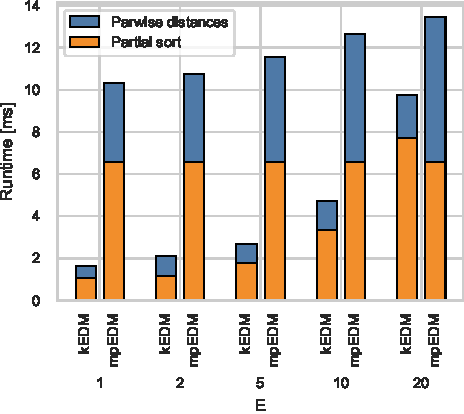
\includegraphics{figs/breakdown_knn_v100}
    \caption{Breakdown of kNN runtime on V100 ($L$=10,000)}%
    \label{fig:breakdown-knn-v100}
\end{figure}

\begin{figure}
    \centering
    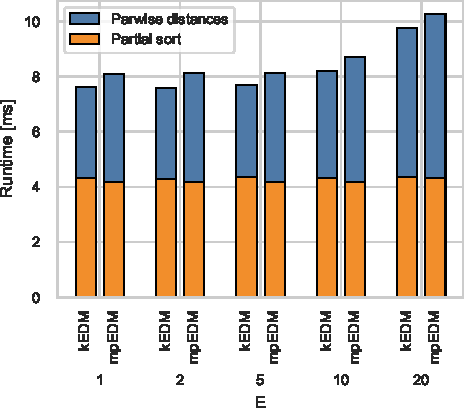
\includegraphics{figs/breakdown_knn_epyc}
    \caption{Breakdown of kNN runtime on EPYC 7742 ($L$=10,000)}%
    \label{fig:breakdown-knn-epyc}
\end{figure}

\begin{figure}
    \centering
    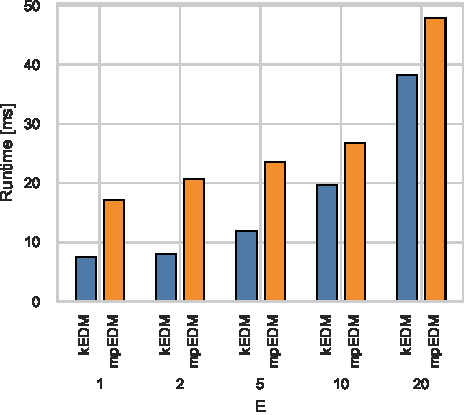
\includegraphics{figs/runtime_lookup_epyc}
    \caption{Runtime of lookups on EPYC 7742 ($L$=10,000, $N$=10,000)}%
    \label{fig:breakdown-lookup-epyc}
\end{figure}

\begin{figure}
    \centering
    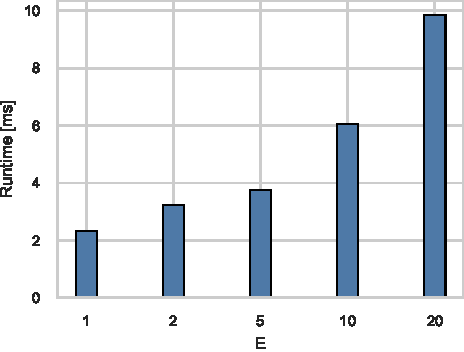
\includegraphics{figs/runtime_lookup_v100}
    \caption{Runtime of lookups on V100 ($L$=10,000, $N$=10,000)}%
    \label{fig:breakdown-lookup-v100}
\end{figure}

\subsection{Efficiency}

To assess the efficiency of our implementation, we conducted a roofline
analysis~\cite{Williams2008} of our kernels. The compute and memory ceilings
on each platform were measured using the Empirical Roofline Toolkit (ERT)\footnote{\url{https://bitbucket.org/berkeleylab/cs-roofline-toolkit/}} 1.1.0.
Since ERT fails to measure the L1 cache bandwidth on GPUs, we used the
theoretical peak performance instead. We followed the methodology presented
in~\cite{Yang2020a,Yang2020b} to measure the arithmetic intensity and the
attained FLOP/s. Nvprof 10.1 and likwid~\cite{Treibig2010} 5.0.1 were used to
collect the required metrics on GPU and CPU, respectively.

% 1.38*80*32*4/1024 = 13.8 TiB/s
% (frequency)*(# of SMs)*(bank size)*(bank width)

\begin{figure}
    \centering
    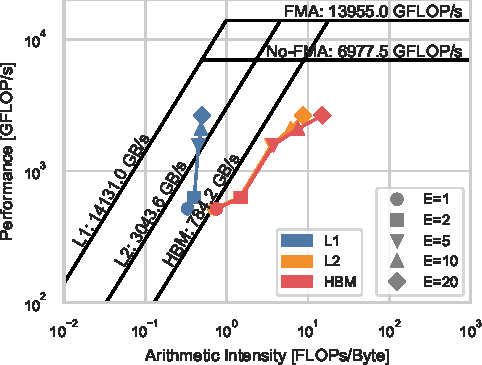
\includegraphics{figs/roofline_distances_v100}
    \caption{Roofline analysis of pairwise distance kernel on V100 ($L$=10,000)}%
    \label{fig:roofline-distances-v100}
\end{figure}

\begin{figure}
    \centering
    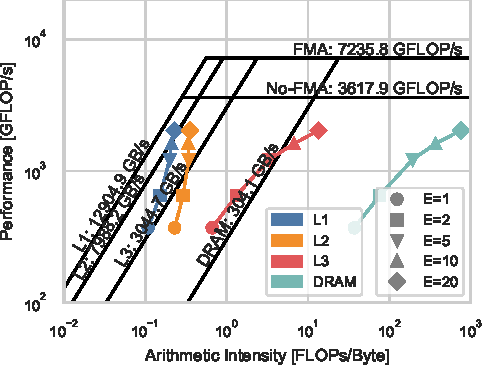
\includegraphics{figs/roofline_distances_epyc}
    \caption{Roofline analysis of pairwise distance kernel on EPYC 7742 ($L$=10,000)}%
    \label{fig:roofline-distances-epyc}
\end{figure}

\begin{figure}
    \centering
    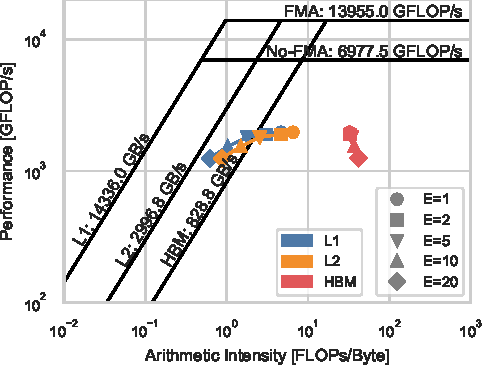
\includegraphics{figs/roofline_lookup_v100}
    \caption{Roofline analysis of lookup kernel on V100 ($L$=10,000, $N$=10,000)}%
    \label{fig:roofline-lookup-v100}
\end{figure}

\begin{figure}
    \centering
    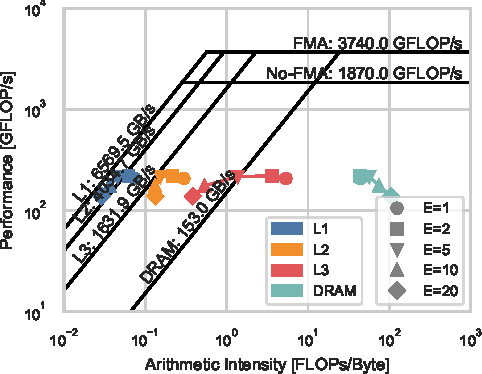
\includegraphics{figs/roofline_lookup_epyc}
    \caption{Roofline analysis of lookup kernel on EPYC 7742 ($L$=10,000, $N$=10,000)}%
    \label{fig:roofline-lookup-eypc}
\end{figure}

\section{Conclusion \& Future Work}

\section*{Acknowledgements}
This work was supported by JSPS KAKENHI Grant Number JP20K19808 (KT) and an
Innovation grant by the Kavli Institute for Brain and Mind (GMP).

\bibliographystyle{IEEEtran}
\bibliography{references}

\end{document}
